\documentclass[11pt,a4paper]{article}
\usepackage[pdftex]{graphicx}
\usepackage[utf8]{inputenc}
\usepackage[francais]{babel}
\begin{document}
\title{Rapport de TP SoC/Cache}
\author{Binôme:}
\maketitle
\section{Rappels et questions de cours}
    \subsection{Question 1 :}
Les mécanismes de mémoire cache se base sur le principe de localité qui dit que le code et les données des programmes ne sont pas utilisées de manière uniforme. On constate souvent que 10\% du code d'un programme contribue à 90\% des instructions exécutées. On distingue deux types de localité : \\

\begin{itemize}
    \item Temporelle qui indique que des éléments auxquels on a eu accès récemment seront probablement utilisés dans un futur proche.
    \item Spatiale qui indique que des éléments proches ont tendances à être référencés à des instants proches.
\end{itemize}

    \subsection{Question 2 :}
L'avantage des caches associatif par rapport aux caches à correspondance direct est qu'ik permet une grande souplesse et une efficacité pour gérer les lignes de manière optimale en terme de succès d’accès. \\

Et l'inconvénient de ce type de cache que l'on doit au pire parcourir toutes les lignes du cache pour savoir si la
ligne cherchée s’y trouve ou pas.
    
    \subsection{Question 3 :}
Les trois types de défaut de cache qui peuvent se produire dans un cache associatif sont : \\

\begin{itemize}
    \item Défauts de première référence (compulsory misses) : À la première référence à un bloc, celui-ci doit être chargé dans le cache. Ces défaut sont en quelque sorte inévitables.
    \item Défauts de capacité (capacity misses) : Ces défauts sont dû au fait que le cache ne peut pas contenir tous les blocs référencés pendant l'exécution du programme. Le nombre de ces défauts peut être réduit en augmentant la taille du cache.
    \item Défauts de conflit (conflict misses) : Ces défauts interviennent en plus des deux précédents types. Un bloc a pu être chargé puis enlevé du cache car d'autres blocs avec le même indice ont été chargés. Le nombre de ces défauts peut être réduit en augmentant l'associativité du cache.
\end{itemize}
    
    \subsection{Question 4 :}


    
\section{Mesures}
\begin{figure}[htbp]
  \centering
  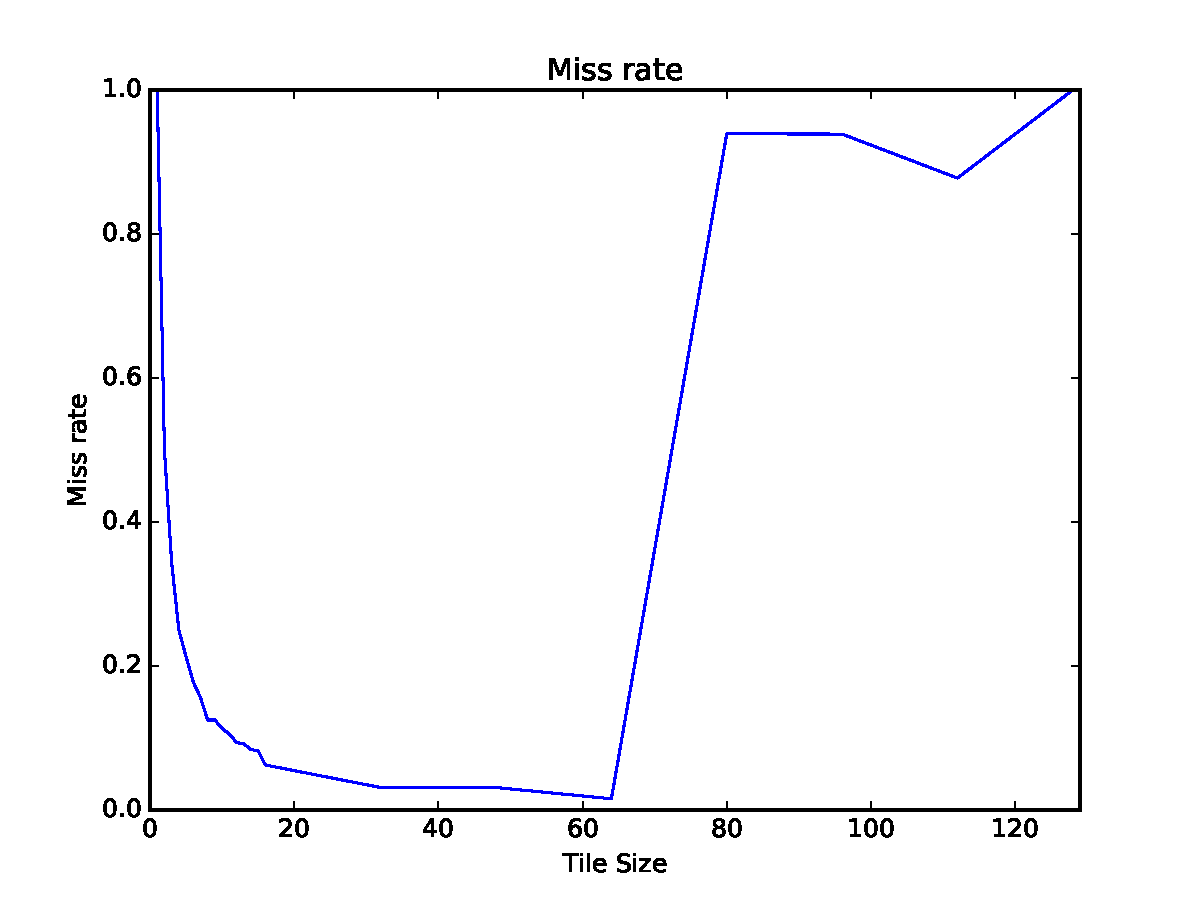
\includegraphics[width=0.9\linewidth]{../res/expe_simple}
  \caption{Alpha=0}
  \label{fig:0}
\end{figure}
 \begin{figure}[htbp]
   \centering
   \includegraphics[width=0.9\linewidth]{../res/expe_simple_OBL}
   \caption{Alpha=0}
   \label{fig:1}
 \end{figure}
\begin{figure}[htbp]
  \centering
  \includegraphics[width=0.9\linewidth]{../res/expe_simple_1}
  \caption{Alpha=0}
  \label{fig:0}
\end{figure}
 \begin{figure}[htbp]
   \centering
   \includegraphics[width=0.9\linewidth]{../res/expe_simple_1_OBL}
   \caption{Alpha=0}
   \label{fig:1}
 \end{figure}
\end{document}